%%%%% this line is 80 chars wide, please don't make longer lines %%%%%%%%%%%%%%%
\documentclass[nocopyrightspace,11pt,authoryear,preprint]{sigplanconf}

%\documentclass[a4paper,11pt]{article}

%\usepackage[francais]{babel}

%\usepackage[utf8]{inputenc}  
%\usepackage[T1]{fontenc}

\usepackage{graphicx}
\usepackage{hyperref}
\usepackage[final]{listings}
\usepackage{setspace}
 %http://texblog.org/tag/setspace/
%http://texblog.org/2011/09/30/quick-note-on-line-spacing/
	%\singlespacing
	%\onehalfspacing
	%\doublespacing

\begin{document}

%\onehalfspacing

\title{Representation of auditory signals by neuronal spike trains}
\subtitle{Bachelor project report} 

\authorinfo{Ma\"elle Colussi}
           {Computational Neuroscience Laboratory (LCN) - EPFL}
					 {Responsible professor: Prof. Wulfram Gerstner, 
					Responsible assistant : Moritz Deger}
\maketitle

\section{Introduction}
%%%%% this line is 80 chars wide, please don't make longer lines %%%%%%%%%%%%%%%
The neuronal representation of sound is the result of the encoding of acoustic 
signals done through the peripheral auditory system. 
The spike trains resulting from this encoding are influenced, 
among other factors, by the refractory period of the 
auditory nerve fibers. 
We learn, for example, in \cite{AvissarPapier} that for the encoding of pure tones, 
the time-spike precision depends in part on the ratio of  
the refractory period to the stimulus period. 
We also know from the research of Berry and Meister described 
in \cite{BerryMeister} that the refractoriness of neurons may make their signals 
more reliable for temporal precision. 
Then, in \cite{Deger}, processes with refractoriness were studied 
and predictions 
were made for Fourier coefficients of response when the stimulus is a pure tone.%%

This project has for purpose to go further in the study the effects of 
the refractoriness on the spike-trains resulting from encoding in the peripheral 
auditory system.  
First, it will study this effect on an ad-hoc computation made on spike trains,  
the rate-modulation depth, for four kinds of stimuli.
Then, it will see if their Fourier coefficients match the predictions
of \cite{Deger}, for a modulated pure tone stimulus. 
Since we have phase-locking for a modulated pure tone stimulus 
as we have in the non-modulated one, we expect the same kind of effect of refractory 
period on the response.



%we have better entrainment of spike trains and often also better precision 
%in time encoding. 
%%%

%This project studied the effects of this neural property 
%on the resulting encoded spike trains. 

For this aim, a model of the peripheral auditory system was used
\cite{Model1, Model2, Model3}, in which the refractory period can be modified. 
Virtual experiments were run on the two versions of the model and the resulting 
spike trains were compared to see the influence of the refractory period. 
Before going any deeper on the model, we should remind us some things 
about the auditory system.

%Acoustic signals are encoded as spike trains by auditory nerve fibers. The time-dependent firing rate and other aspects of spike train statistics depend, among other things, on the refractory period of the nerve fibers. This project aims to understand the influence of the refractory period on the neuronal representation of sounds.

%A phenomenological model of the peripheral auditory system [1,2] will be used to perform virtual experiments. The model allows to modify the refractory period of the nerve fibers. The responses of the model to a selection of auditory stimuli will be recorded and characterized as a function of the neuronal refractory period. If time permits, specific theoretical predictions like frequency doubling [3] will be tested.


\section{The Auditory System}
%%%%% this line is 80 chars wide, please don't make longer lines %%%%%%%%%%%%%%%
The "Auditory Neuroscience" book \cite{AuditoryNeuroscience} tells us in the 
chapter two what is important for us here to know. 

The peripheral auditory system has (generally air) pressure as input, 
and spike trains as output. We will go through the parts of the ear, with help 
of \autoref{fig:ear}. 

Let us consider first the external ear. There the pressure signals come through
 the ear canal and make the eardrum vibrate. 
This takes us to the medium ear. 
The vibration is propagated throughout it by three ossicles : malleus, incus 
and stapes. The farthest part from the external ear of the stapes touches the 
boundary of the cochlea, on the oval window, in the inner ear, 
and makes vibrate the liquid we find in it. 
The cochlea forms an interface between this mechanical vibration 
and the neural signal that will go through the auditory nerve 
(VII nerve on \autoref{fig:ear}).
%\begin{figure*}[placement specifier] %* for 2 columns prob
%... figure contents ...
%
%\end{figure}
%http://en.wikibooks.org/wiki/LaTeX/Floats,_Figures_and_Captions

%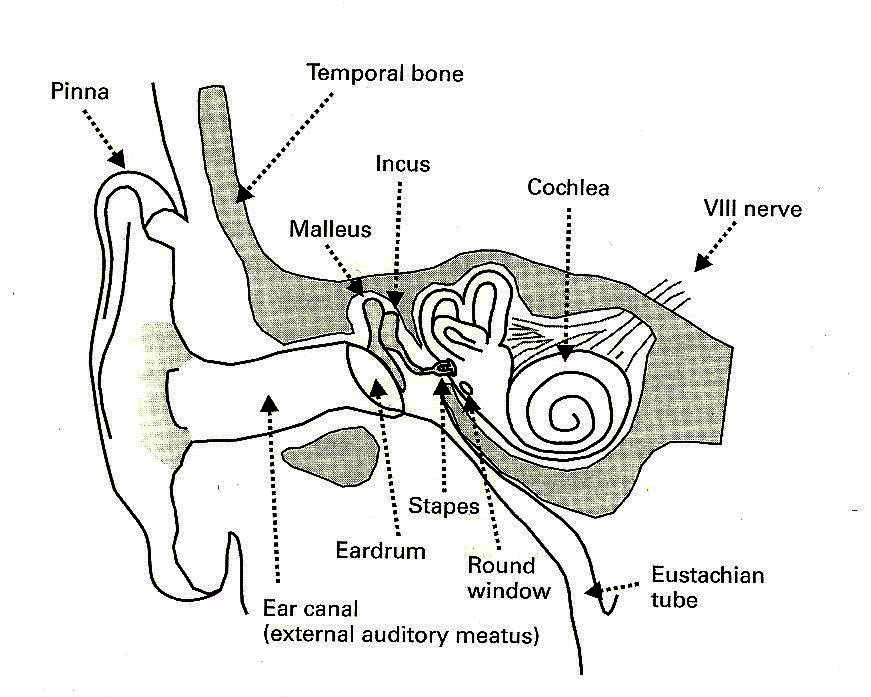
\includegraphics[width=0.45\textwidth]{images/ear-aud52-level.jpg}

\begin{figure}[h]
	\centering
	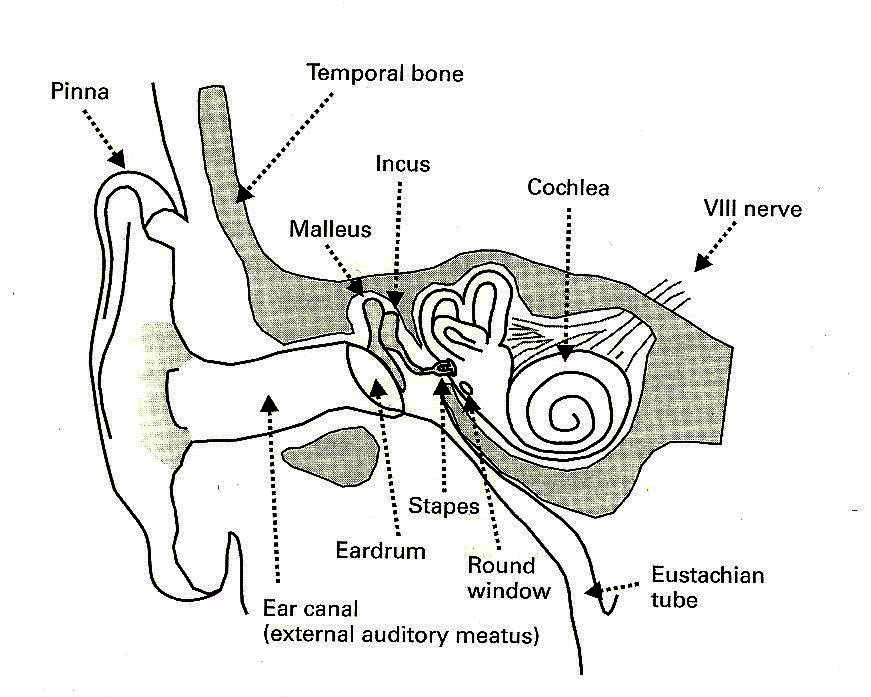
\includegraphics[width=0.45\textwidth]{images/ear-aud52-level.jpg}
	\caption{Peripheral auditory system (\cite{AuditoryNeuroscience} p.52 )}
	\label{fig:ear}
\end{figure}

We will speak more about this interface below. But first we should see 
more about the vibration of the cochlea. 
The cochlea is a tube that has two main compartments which are placed on top of 
each other and separated throughout the cochlear tube by  
the basilar membrane,  except at the far end of it where they are joined, 
as you can see on \autoref{fig:ucochlea}.

%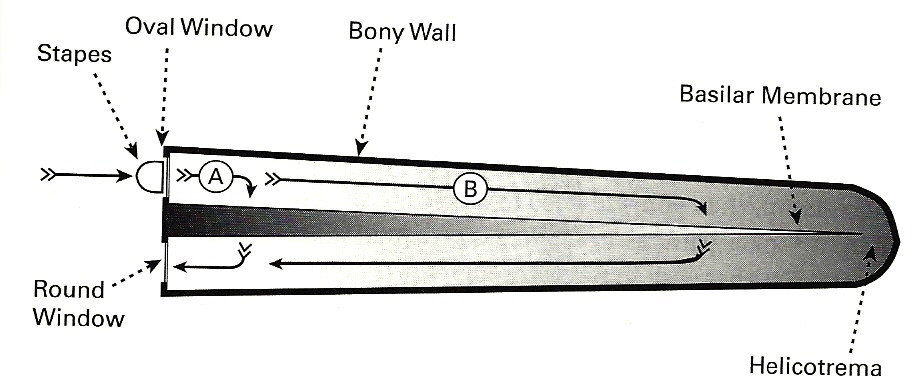
\includegraphics[width=0.45\textwidth]{images/cochlea-aud55-level.jpg}

\begin{figure}[h]
	\centering
	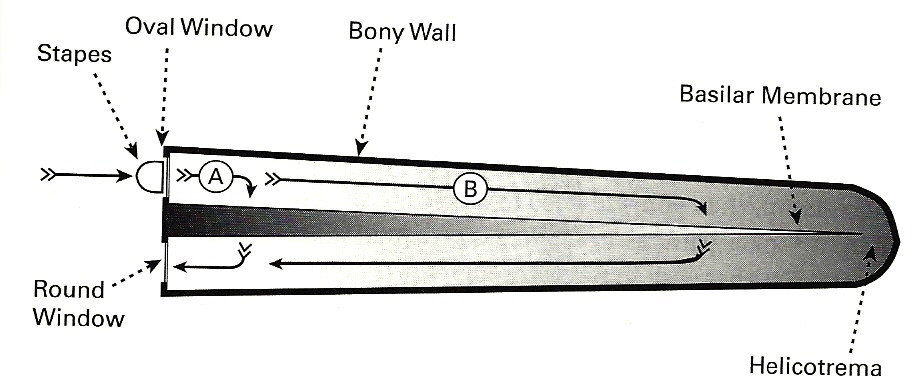
\includegraphics[width=0.45\textwidth]{images/cochlea-aud55-level.jpg}
	\caption{Unrolled cochlea (\cite{AuditoryNeuroscience} p.55 )}
	\label{fig:ucochlea}
\end{figure}

%put that one page before the page it should appear on :
%http://www.andrewjpage.com/?archives/48-Figure-spanning-2-columns-in-Latex.html
\begin{figure*}[ht]
	\centering
  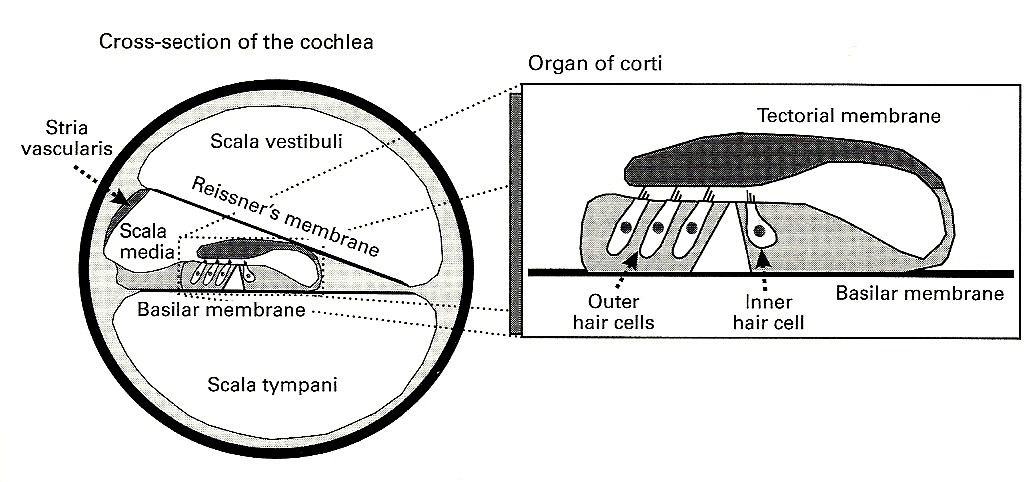
\includegraphics[width=0.75\textwidth]{images/corti2-aud65-level.jpg}
	\caption{Organ of Corti (\cite{AuditoryNeuroscience} p.65 )}
	\label{fig:corti}
\end{figure*}

A vibration that comes will try to propagate through the basilar membrane from 
the upper compartment to the other. When doing that, it will not make all 
the parts of the basilar membrane vibrate at the same intensity. 
In fact, the cochlea is like a "biological Fourier analyzer" according to the book. 
The frequency content of vibrations is decomposed and each frequency has its 
"favorite" place in the cochlear coiled tube that it makes vibrate particularily. 
The part of the basilar membrane that is the first we can see vibrating, 
when we gradually put on the volume of a pure tone of frequency f, is said to be of 
"characteristic frequency" f. Near the oval window, the characteristic 
frequencies are high, and as we go to the tip of the tube, 
the characteristic frequency becomes lower.

Throughout the cochlear tube, we have the organ of Corti, which is the interface
about which an allusion was made above in the text. We will use \autoref{fig:corti} to illustrate our purpose.

%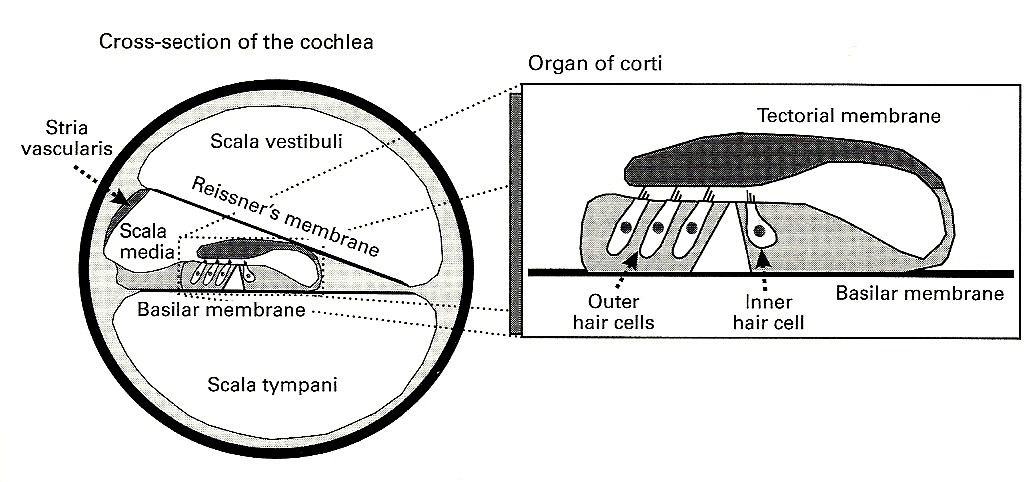
\includegraphics[width=0.45\textwidth]{images/corti2-aud65-level.jpg} %do a better one : perhaps two parts ?



The upper compartment of the cochlea is in fact in two parts separated by a membrane.
The scala media, where we find the organ of Corti, has a higher 
concentration of potassium cations. We have as consequence a polarization between
the liquid of the scala media and the inner hair cells. 
When the basilar membrane vibrates, the tectorial membrane does 
that also and that makes the liquid move. 
These movements has as consequence the deflection of the stereocili 
of the inner hair cells, and when this happens, some potassium ions of the 
scala media go into the inner hair cells (IHC), and we have a depolarization.
%The outer hair cells undergo the same process, but , for their part, have a role of amplificator for the liquid movements. %% word about ohc ?
We can see that in \autoref{fig:transd}.
This has as consequence that some glutamate is leaked in synapses %glutamate checked : p75
between the IHC and the auditory nerve fibers, what excites these fibers 
and make them perhaps have some spikes.

%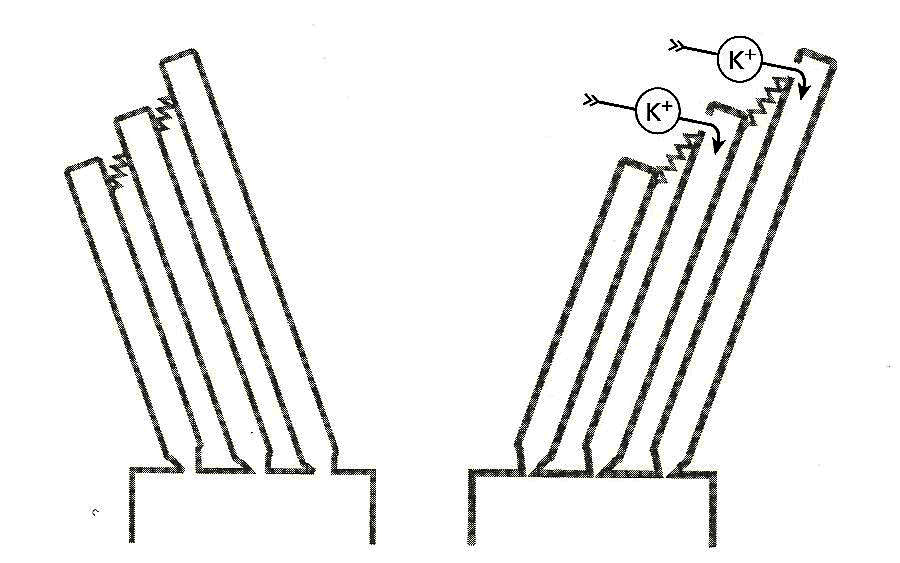
\includegraphics[width=0.45\textwidth]{images/hctransd-aud66-level.jpg}

\begin{figure}[h]
	\centering
  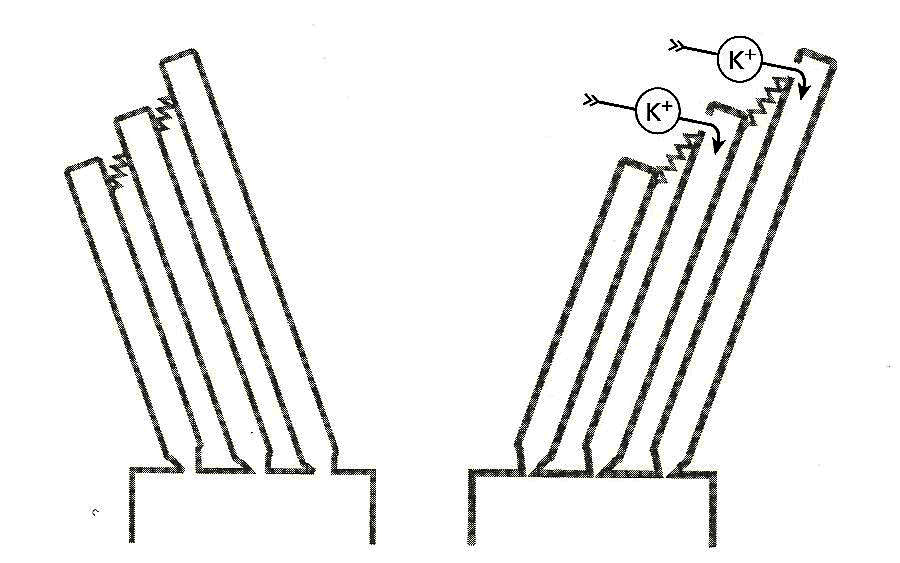
\includegraphics[width=0.45\textwidth]{images/hctransd-aud66-level.jpg}
	\caption{Transduction (\cite{AuditoryNeuroscience} p.66 )}
	\label{fig:transd}
\end{figure}

\section{Model}
%%%%% this line is 80 chars wide, please don't make longer lines %%%%%%%%%%%%%%%
Let us now intriduce the model of the peripheral auditory system
\cite{Model1, Model2, Model3}, which was used to run experiments in this project. 

We will not go into the details of the model, but from the use of it. 
You can see in \autoref{fig:modelsch} the schematic of the model.
It is a complicated cascade of linear and non-linears filters.


%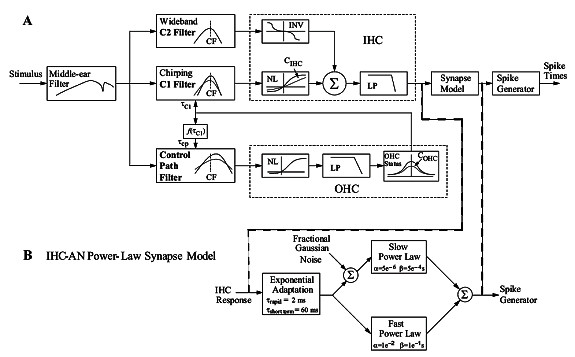
\includegraphics[width=0.45\textwidth]{images/www-bme-rochester-edu-schematicDiagram-level.jpg} %put in auditsys

From the user point of view, the model consists of two main functions 
that are called "catmodel\_IHC" and "catmodel\_Synapse".
 Their prototype, in MatLab language, are

\texttt{vihc = catmodel\_IHC(pin, CF, nrep, tdres, reptime, cohc, cihc);}

and

\texttt{[synout, psth] = catmodel\_Synapse(vihc, CF, nrep, tdres, fibertype, implnt);}

like specified in the "catmodel.m" file of the model. 
Let us go deeper into what each parameter and return value of these functions means.

The first function, \texttt{catmodel\_IHC}, takes as parameters 
a sound pressure stimulus vector (\texttt{pin}, in Pa), sampled at some sampling rate 
that is the inverse of the bin size specified in \texttt{tdres}, and 
the characteristic frequency (\texttt{CF}, in Hz) 
of the IHC and for which we want to know the potential 
(\texttt{vihc}, in Volt) when stimulated. 
This latter (\texttt{vihc}) is what is returned by the function. 
\texttt{reptime} is the time for one repetition of the stimulus, 
and \texttt{nrep} is the number of repetions we want to be run. 
The parameters \texttt{cohc} and \texttt{cihc} represents the damages on respectively 
the outer hair cells and inner hair cells in the simulation (not used in this project).
\texttt{vihc} will contain the IHC potential for every repetition 
after the function has been run.

The second function, \texttt{catmodel\_Synapse}, 
takes the IHC potential returned by \texttt{catmodel\_IHC}, 
with the same sampling rate, so the same \texttt{tdres}, which is also here the bin size
of the PSTH returned by the function (\texttt{psth}). 
The PSTH will be computed according to the specified number of repetitions (\texttt{nrep}).
The synapse output of the IHC (\texttt{synout}) is also returned by the function.
The \texttt{fibertype} parameter is used to tell the model which nerve fiber type
we "test" with the stimulus, distinguished by their spontaneus rate (SR) : 
low, medium or high. 
%(low : $<$ 1 spike/s, medium : $<$ 18 spike/s, high: 20-50 spike/s, 
%according to \cite{AuditoryNeuroscience}). %82
Finally, \texttt{implnt} is used to indicate the precision we want in the simulation 
for the power-law functions in the model.

As an example of what kind of result the model can give,
in \autoref{fig:g4tonestep} you can see some graphs that represents the steps of a 
simulation of a pure tone step stimulus.
A nerve fiber with high SR with a 1 kHz characteristic frequency 
was chosen.

%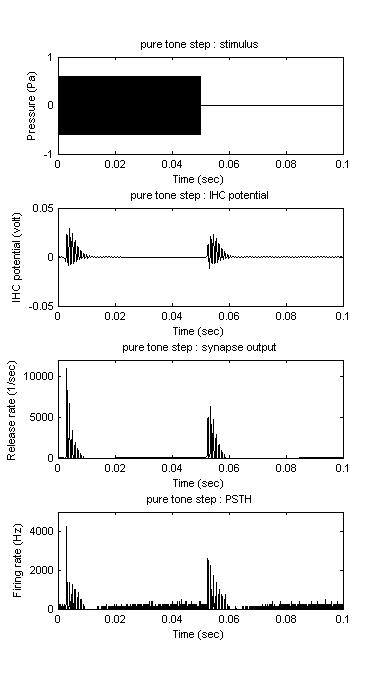
\includegraphics[width=0.45\textwidth]{images/g4-tonestep-column3.jpg}

\begin{figure}[h]
	\centering
	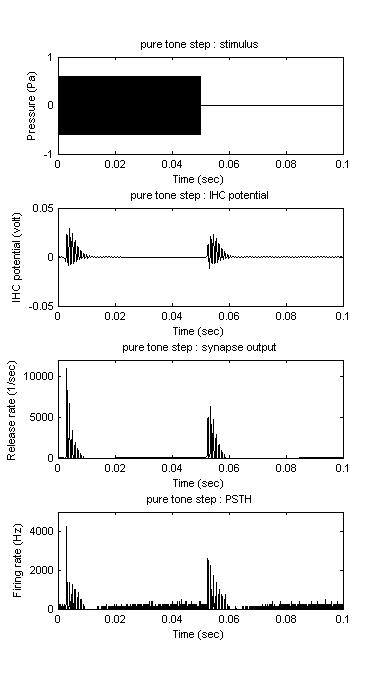
\includegraphics[width=0.45\textwidth]{images/g4-tonestep-column3.jpg}
	\caption{Example of model results (\cite{Model1})}
	\label{fig:g4tonestep}
\end{figure}

The first graph is a representation of one period of the stimulus, 
sampled at 100'000 Hz (so with bins of 0.01 ms size), at 84dB SPL.
The stimulus, as given to the model as \texttt{pin}, was this period of 100 ms repeated 800
times : a pure tone step. 
The frequency of the pure tone is so high here (10 kHz) that we cannot see its sinusoid.
On the second graph, you can see the IHC potential from the first function
in response of the last repetition of the stimulus 
(with dependencies on the preceding periods included).
The third graph shows a part of the synapse output given by \texttt{catmodel\_Synapse}, 
for the same period as for the potential of IHC.
The fourth graph represents the peristimulus time histogram (PSTH).

For the project, the code of the model has been modified to put to zero 
the absolute refractory period (ARP) of nerve fibers. 
This transformation was done in the spike generator 
part of the model (see in \autoref{fig:modelsch} the step pointed by the arrow).
After that, the spike trains with and without this refractory period could be compared.

In \autoref{fig:psthcomp} you can see an example of a graph
where are drawn two periodograms, calculated from the PSTH given by the model 
(either modified or not), for another stimulus as before, a pure tone
which is not modulated.

%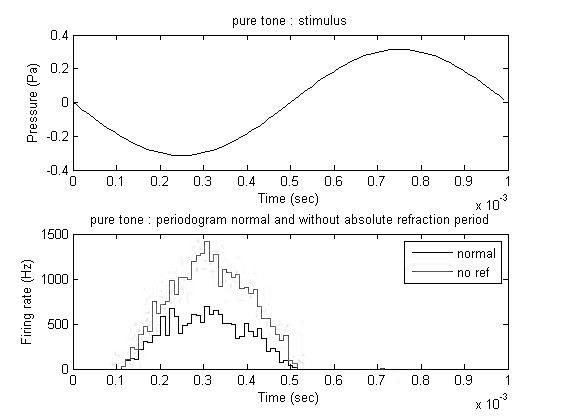
\includegraphics[width=0.45\textwidth]{images/stim-psth-puretone-bw2.jpg}

\begin{figure}[h]
	\centering
	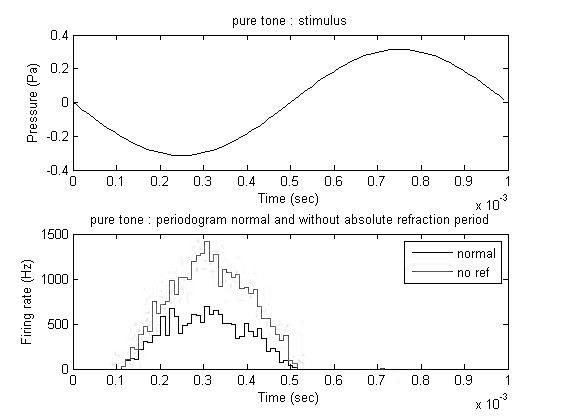
\includegraphics[width=0.5\textwidth]{images/stim-psth-puretone-bw2.jpg}
	\caption{Periodogram with and without refractory period for the stimulus of period above}
	\label{fig:psthcomp}
\end{figure} 

In \autoref{fig:psthcomp}, first graph, you can see one period of the stimulus, 
a 1 kHz pure tone, at 84dB SPL.
The second graphs shows the periodogram with and without absolute refractory period.
We can see phase-locking for the two periodograms : spikes occur preferentially 
for a specific phase of the stimulus cycle. We see that here the phase caracteristics 
 seems not to change when the refractory period changes.
This simulation was done with a medium SR nerve fiber, 
with 1 kHz characteristic frequency and 100 ms bin size.
We will see now describe the results of the project.

%\begin{lstlisting}[caption={},captionpos=b]{}
%\end{lstlisting}

%\texttt{tdres} 

\section{Results}
%%%%% this line is 80 chars wide, please don't make longer lines %%%%%%%%%%%%%%%

\subsection{Rate modulation depth}

\begin{figure*}[ht]
	\centering
  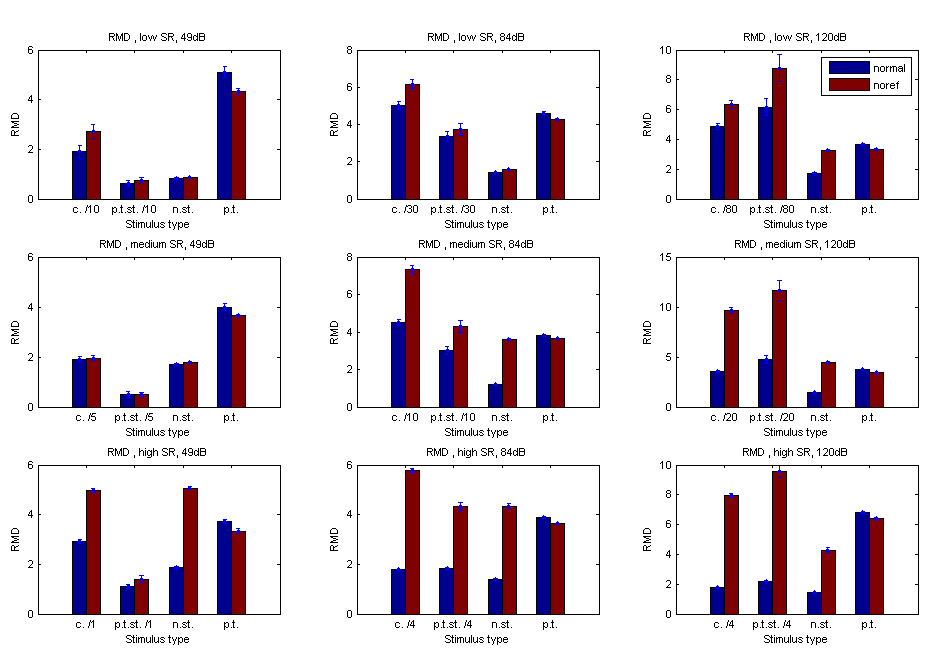
\includegraphics[width=\textwidth]{images/rmds9.png} %or jpg ?; TODO have a better one, and crop it with Paint, see if ok when printed
	\caption{RMD values for different SR fibers and intensities. Experiment labels are abbreviated 
	(c. for click, p. t. st. for pure tone step, n. st. for noise step, p. t. for pure tone).
	Some RMD results had to be scaled to fit properly in the graph and the scaling factor is written in the legend of the x-axis.
	From left to right, we have sound intensities : 49 dB, 84 dB, 120 dB,
	from top to bottom, we have fiber types : low SR, medium SR and high SR.}
	\label{fig:rmds}
\end{figure*}

For the first part of the project, an ad-hoc measure called rate 
modulation depth (RMD) was used to quantify differences between encoding 
of acoustic signal with and without an absolute refractory period (ARP) of the auditory nerve.

Four kinds of experiments where run and the average RMD was calculated 
for each of them, 
with each type of nerve fiber, and three different sound intensities : 
49 dB SPL, 84 dB SPL and 120 dB SPL (49 dB : average home, rainfall; 84 dB : busy road; 120 dB : threshold of discomfort, possible hearing loss) 
% TODO
%http://www.sengpielaudio.com/TableOfSoundPressureLevels.htm; citate ?
%http://noiselimiters.co.uk/buy/noise-levels-what-is-noise.php
to have an overall view of the effects.
For each virtual experiment, the bin size was 0.01 ms, the characteristic frequency was 1 kHz, 
there was no damage on IHC or OHC, and we told the model to use the built-in approximations 
for power-law function calculations.

The four experiments were clicks, pure tones, noise steps and pure tone steps.
The clicks were rarefaction clicks (negative pressure excursion) of 0.1 ms and sufficient time was waited between 
two of them to avoid influence from one to the other.
The two step stimuli had a period of 100 ms and in the first half of the period 
there was noise or pure tone signal, and in the second half there was 0 Pa as pressure.
The noise for the noise step was composed of random normal variables divided 
by the square root of the bin size (gaussian white noise).
The pure tone of the pure tone step was of 10 kHz frequency.

The rate modulation depth (RMD) was defined as 

\begin{equation}\label{rmdformula1} RMD =  \frac{m - b}{b}\end{equation}
%http://www.math.uiuc.edu/~hildebr/tex/displays.html

%for pure tone steps and noise steps, and as
%
%\begin{equation}\label{rmdformula2} RMD = \frac{< m >}{< b >} - 1\end{equation}
%
for clicks and pure tone steps,
where $m$ was 
the maximum of the periodogram of the encoded sounds when converted in 2 ms bins.
The meaning of the $b$ depended on the stimulus. 
For the clicks it corresponded to the mean response to a 0 Pa pressure signal,
 with same number of repetitions than for the click stimulus. 
For the noise step, the baseline is the value of the periodogram just before the second 
half of the period, so just before the stimulus onset,
 in 10 ms bins. 
The baseline for the pure tone step was the mean of PSTH values
of a response to a pure tone of the frequency used for the stimulus (10 kHz),
after the IHC were saturated (as could be seen in the potential, 
which stays constant because it has not the time 
to be depolarized between two periods of the stimulus). 
The periodogram was computed from the same number of repetitions as for the pure tone step stimulus.
For the pure tone, the baseline was chosen as the mean of the periodogram.
For pure tones and noise steps, for each repetition the RMD was calculated and the final result is the mean, whereas
for clicks and pure tone steps $b$ and $m$ where found separately and their means where then used for the RMD calculation.
%When baselines for clicks and for pure tone step where computed, 
%we took attention to the fact that the number of repetitions of stimulus
%for the used periodogram should correspond to the one for the periodogram used for 
%calculating the maximum. 
%It gives then an equivalent RMD as if we had divided each periodogram by 
%their own number of repetitions.

\autoref{fig:rmds} displays RMD values as obtained in our virtual experiments, 
for several fiber types and sound intensities. 
Error bars for noise steps and pure tones are standard deviation of the mean of the RMDs calculated for each repetition of the stimulus. 
For clicks and pure tone step, the error bars are of value $\sigma_{< RMD >}$. To find this value, the standard deviation of the means of $m$ and $b$ were calculated and then propagated for the division with \autoref{errorprop}.

\begin{equation}\label{errorprop}\frac{\sigma_{< RMD >}}{|<RMD>|}= \sqrt{\left(\frac{\sigma_{< m >}}{< m >}\right)^2 + \left(\frac{\sigma_{< b >}}{< b >}\right)^2} \end{equation}
 
As displayed on \autoref{fig:rmds}, overall effects are these:
for clicks, pure tone steps and noise steps, the RMD without absolute refractory
period is bigger than for the normal case, and it is the opposite for pure tones.

%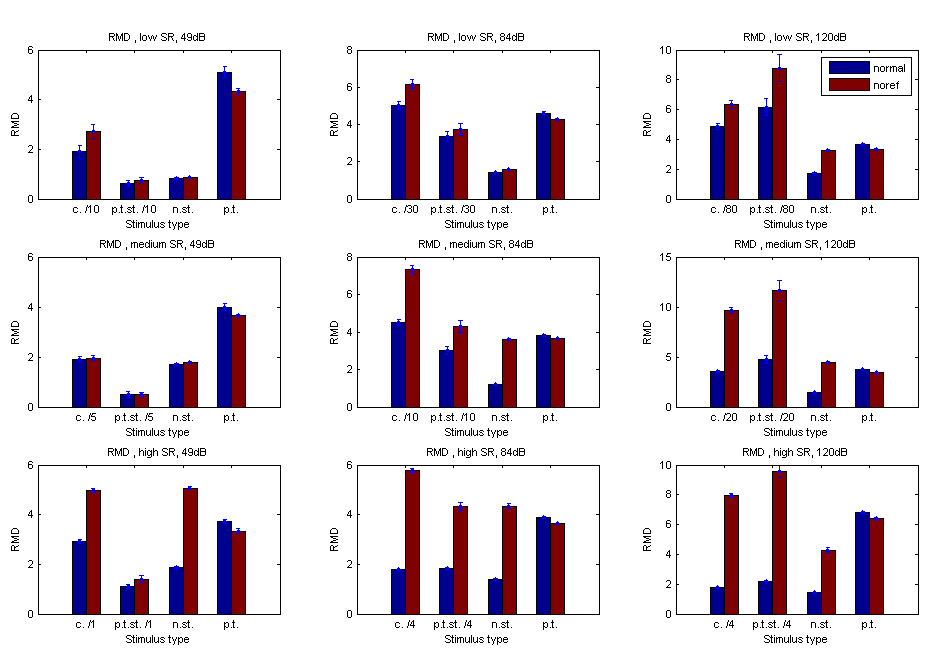
\includegraphics[width=0.45\textwidth]{images/rmds9.jpg}%put higher

We may explain the first finding because, first, we are in presence of a highly 
non-linear system and, 
secondly, the three stimuli for which the RMD without ARP is bigger, 
are stimuli with very sudden changes. 
In fact, the click can be seen as an approximation of a delta function, 
which corresponds to a broad-band stimulus. 
Also, sudden steps excite a wide range of frequencies, 
which make many non-linearities of the system contribute to the response.

%which induces a peak in the periodogram just after it, 
%and for the steps we have suddenly a signal for some time and suddenly, 
%we have no more of it, and that repeatedly, and at each of these changes, 
%we have a peak in the periodogram. 
%These peaks are then the ones which are used in the RMD computation as the maximum.
%In consequence, this RMD result can be interpreted like that : the absolute refractory period 
%seems to be able to lower the intensity of the strong response transient induced 
%when these kind of sudden changes happens.

The second finding that RMD is lower for pure tones without ARP, 
may be explained by the fact that we have less 
interactions between frequencies in the non-linear system up to the spike generator, 
in the model,
and the effects of ARP are strong enough to be seen.

\subsection{Response according to frequencies of modulated pure tones}

In \cite{Deger}, predictions are made for the absolute value (norm) and angle of the Fourier coefficients 
(harmonics 0, 1, 2 and 3) of response of stochastic point processes with refractory period,
to sinusoidal stimuli, as a function of the frequency. 
This case roughly corresponds to a tone with a high frequency carrier function, 
modulated by a low frequency oscillation. 
In fact, the inner hair cells will not be able to follow the carrier frequency 
and they will excite the nerve with a synaptic release rate dominated by the modulation.

The product of the absolute refractory period $d$ and the modulation frequency $f$,
determines the response spectrum, as shown in \autoref{fig:prednorm} (norm of Fourier coefficient) and 
\autoref{fig:predangle} (angle). Here $d$ was 80 ms. 
In the graphs, the black ligns are for harmonic 0, dark gray for 1, mid gray for 2, light gray for 3.
$\beta_k$ is the k harmonic of the output. 


%\includegraphics[page=...,viewport=llx lly urx ury,clip]{pdf-file}

\begin{figure}[h]
	\centering
	\includegraphics*[page=4,viewport=308 567 441 617]{images/Deger2010.pdf} %x, y, x, y
	\caption{Predictions for norm (\cite{Deger}  their fig. 3 (c))}
	\label{fig:prednorm}
\end{figure}

\begin{figure}[h]
	\centering
	\includegraphics*[page=4,viewport=433 567 566 619]{images/Deger2010.pdf} %x, y, x, y
	\caption{Predictions for angle (\cite{Deger} their fig. 3 (d))}
	\label{fig:predangle}
\end{figure}
%http://tex.stackexchange.com/questions/40658/extracting-image-from-pdf-to-use-in-latex-document
%pdfimages [options] <PDF-file> <image-root>, on Linux
%http://www.artofproblemsolving.com/Wiki/index.php/LaTeX:Pictures
%http://ctan.org/pkg/graphicx

\begin{figure*}[ht]
	\centering
  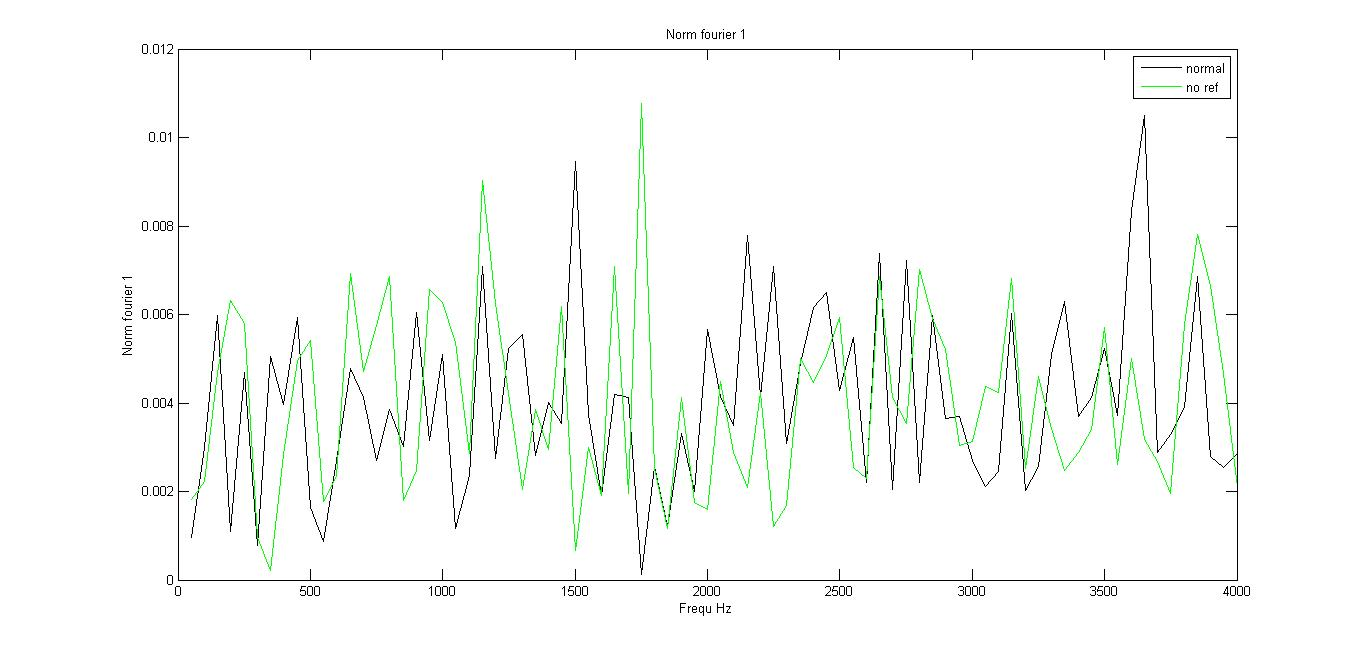
\includegraphics[width=\textwidth]{images/norm1.jpg}
	\caption{Norm of first harmonic of response to a modulated pure tone, in function of modulation frequency}
	\label{fig:norm1}
\end{figure*}

To see if the predictions are coherent with the model of the peripheral auditory 
system, experiments with modulated pure tone were run. 
The carrier frequency used was 10 kHz, the modulation frequency varied from 50 Hz to 4000 Hz
with steps of 50 Hz. We chose nerve fibers with medium SR, characteristic frequency 5 kHz 
and the stimuli were of intensity 84 dB.
The stimulis $y\left(t\right)$ were calculated like that :

\begin{equation}\label{freqstim} y\left(t\right) = A \left(1+0.5sin \left(2 \pi t f_m \right)\right) sin \left(2 \pi t f_c \right)\end{equation} %TODO %\odot
where $A$ is the amplitude,
$f_m$ is the modulation frequency,
$f_c$ is the carrier frequency.

 
Two seconds of each stimulus were run, 
then, the second half of the PSTH was kept and its $\beta_k$ Fourier coefficients were calculated according the following formula.

\begin{equation}\label{bkformula} \beta_k = \frac{1}{T} \sum_{j= 0}^{\frac{T}{\Delta t}} e^{i \omega k j \Delta t} z \left( j \Delta t\right)\Delta t\end{equation}

where $T$ is the period (1 second here), %1sec pour tous les stimulis. expliquer ?
 $\omega$ is $\frac{2\pi}{T}$,
$\Delta t$ is the bin size (0.01ms),
$z\left(t\right)$ is the PSTH,
and $k$ is the number of the caculated harmonic.

In the model, the absolute refractory period is of 0.75 ms, so mutiples of $1/d$ are near 1333 Hz and 2666 Hz in our experiments.
Sadly, not enough data could be yet calculated to see if the results match the predictions of 
\cite{Deger}. 
As you can see in \autoref{fig:norm1}, after 10'400 repetitions, the results are too noisy to be able to conclude anything. %TODO nr rep
The graph shows the norm of the first harmonic. The other norms and angles graphs are also chaotic, so we do not show them.

%put frequ graph, even if to say : too noisy to see anything
%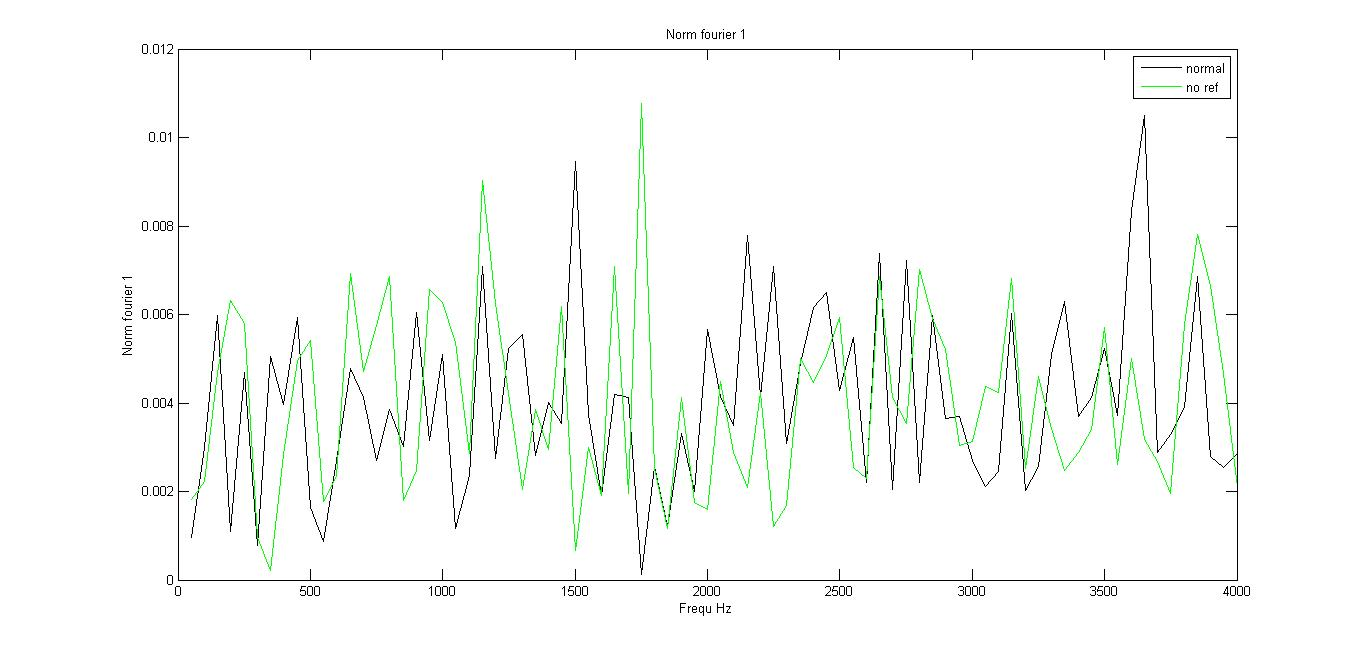
\includegraphics[width=\textwidth]{images/norm1.jpg}











 

\section{Conclusion}
%%%%% this line is 80 chars wide, please don't make longer lines %%%%%%%%%%%%%%%
The rate modulation depth calculation gave interesting results. 
In fact, RMD is a measure of the relative precision of response,
and we found that absolute refractory period increased precision only 
for a specific stimulus (pure tone). %%tell about ref of 2013

For the second part of the project, the results were too noisy to conclude anything.

\bibliographystyle{abbrvnat}
\bibliography{bibliography}

%https://en.wikipedia.org/wiki/BibTeX
%http://en.wikibooks.org/wiki/LaTeX/Document_Structure
%http://en.wikibooks.org/wiki/LaTeX/Floats,_Figures_and_Captions
%\cite{AuditoryNeuroscience} 
%\onecolumn
%\twocolumn

\end{document}
